% This file has been slightly modified from Hans Kestler's original to reflect
% changes in the CinC style file (cinc.cls), in which the width of the text
% columns has been slightly reduced.  Accordingly, the size of figure 2 has
% been reduced so that the entire paper will fit into four pages as in the
% original. --GBM
\documentclass[twocolumn]{cinc}

\usepackage{amssymb}    % Written by Donald Arseneau
\usepackage{amsmath}   % From the American Mathematical Society
\usepackage{multirow}
\usepackage{subfigure}
\usepackage{epsfig}
\usepackage{color}
%\usepackage{mathtools}\usepackage[english,activeacute]{babel}
\usepackage[utf8]{inputenc}
\usepackage{amsmath}
\usepackage{amsfonts}
%\usepackage{hyperref}
\newcommand{\mfhr}{\ensuremath{\overline{FHR}}}
\newcommand{\myred}[1]{\textcolor{red}{#1}}  
\newcommand{\myblue}[1]{\textcolor[rgb]{0,0.14,0.4}{#1}}
\newcommand{\myorange}[1]{\textcolor[rgb]{1,0.56,0}{#1}}

% S�mbolos Matem�ticos.

\newcommand{\fxh}[1]{f_{X|H_#1}}
\newcommand{\fbxh}[1]{f_{\mathbf{X}|H_#1}}


\newcommand{\Mia}{\boldsymbol{a}}
\newcommand{\Mir}{\boldsymbol{r}}
\newcommand{\Mix}{\boldsymbol{x}}
\newcommand{\Miy}{\boldsymbol{y}}
\newcommand{\Miz}{\boldsymbol{z}}


\newcommand{\ba}{\mathbf{a}}
\newcommand{\bc}{\mathbf{c}}
\newcommand{\bk}{\mathbf{k}}
\newcommand{\bn}{\mathbf{n}}
\newcommand{\bp}{\mathbf{p}}
\newcommand{\bq}{\mathbf{q}}
\newcommand{\br}{\mathbf{r}}
\newcommand{\bs}{\mathbf{s}}
\newcommand{\bt}{\mathbf{t}}
\newcommand{\bu}{\mathbf{u}}
\newcommand{\bw}{\mathbf{w}}
\newcommand{\bx}{\mathbf{x}}
\newcommand{\by}{\mathbf{y}}
\newcommand{\bz}{\mathbf{z}}

\newcommand{\bA}{\mathbf{A}}
\newcommand{\bB}{\mathbf{B}}
\newcommand{\bC}{\mathbf{C}}
\newcommand{\bD}{\mathbf{D}}
\newcommand{\bE}{\mathbf{E}}
\newcommand{\bF}{\mathbf{F}}
\newcommand{\bH}{\mathbf{H}}
\newcommand{\bI}{\mathbf{I}}
\newcommand{\bK}{\mathbf{K}}
\newcommand{\bP}{\mathbf{P}}
\newcommand{\bQ}{\mathbf{Q}}
\newcommand{\bR}{\mathbf{R}}
\newcommand{\bS}{\mathbf{S}}
\newcommand{\bT}{\mathbf{T}}
\newcommand{\bU}{\mathbf{U}}
\newcommand{\bV}{\mathbf{V}}
\newcommand{\bW}{\mathbf{W}}
\newcommand{\bX}{\mathbf{X}}
\newcommand{\bY}{\mathbf{Y}}
\newcommand{\bZ}{\mathbf{Z}}
\newcommand{\buno}{\mathbf{1}}

\newcommand{\mcA}{\mathcal{A}}
\newcommand{\mcC}{\mathcal{C}}
\newcommand{\mcD}{\mathcal{D}}
\newcommand{\mcF}{\mathcal{F}}
\newcommand{\mcG}{\mathcal{G}}
\newcommand{\mcH}{\mathcal{H}}
\newcommand{\mcP}{\mathcal{P}}
\newcommand{\mcR}{\mathcal{R}}
\newcommand{\mcX}{\mathcal{X}}
\newcommand{\mcY}{\mathcal{Y}}
\newcommand{\mcZ}{\mathcal{Z}}

\newcommand{\bbR}{\mathbb{R}}


\newcommand{\balpha}{\boldsymbol{\alpha}}
\newcommand{\bbeta}{\boldsymbol{\beta}}
\newcommand{\bdelta}{\boldsymbol{\delta}}
\newcommand{\bgamma}{\boldsymbol{\gamma}}
\newcommand{\bmu}{\boldsymbol{\mu}}
\newcommand{\bphi}{\boldsymbol{\phi}}
\newcommand{\bpsi}{\boldsymbol{\psi}}
\newcommand{\btheta}{\boldsymbol{\theta}}
\newcommand{\bvarphi}{\boldsymbol{\varphi}}
\newcommand{\bPhi}{\boldsymbol{\Phi}}
\newcommand{\bPsi}{\boldsymbol{\Psi}}
\newcommand{\bTheta}{\boldsymbol{\Theta}}

\newcommand{\htheta}{\hat{\theta}}

\newcommand{\hg}{\hat{g}}
\newcommand{\hF}{\hat{F}}
\newcommand{\hG}{\hat{G}}

\newcommand{\bdexp}[1]{\ensuremath{\mathbf{\times 10^{#1}}}}
\newcommand{\dexp}[1]{\ensuremath{\times 10^{#1}}}
\def\sign{\mathop{\rm sign}\nolimits}

\newcommand{\muestra}[2]{\ensuremath{#1_1,#1_2,\ldots,#1_{#2}}}
\newcommand{\muestraa}[1]{\ensuremath{#1_1,#1_2,\ldots}}
\newcommand{\muestral}[2]{\{\muestra{#1}{#2}\}}
\newcommand{\muestraal}[1]{\{\muestraa{#1}\}}

\newcommand{\mpe}[1]{\ensuremath{\langle #1 \rangle}}
\newcommand{\mnorm}[1]{\ensuremath{\| #1 \|}}

%%% Cosas en lat�n




%%Tablas

\newcommand{\mirbd}[1]{\raisebox{-1.5ex}[0pt]{#1}}


%

\begin{document}
\bibliographystyle{cinc}

\title{Physiological Feature Analysis in Heart Rate Turbulence Using LASSO Model}
\author{1}

\maketitle

%%Abstract%%%%%%%%%%%%%%%%%%%%%%%%%%%%%%%%%%%%%%
\begin{abstract}
Heart Rate Turbulence (HRT) is a relevant cardiac risk stratification criterion. It is usually assess by means of turbulence slope ($TS$) and turbulence onset ($TO$) parameters. HRT is known to be affected by several physiological factors, mainly heart rate (HR) and coupling interval ($CI$). The physiological hypothesis accepted is the baroreflex source of the HRT. However, several studies showed different results about the relationship between CI and HRT parameters. Our aim was to propose a complete LASSO model using $CI$ and sinus cardiac length ($SCL$), their powers and an interaction term as explanatory variables to account for the physiological dynamic of the $TS$ parameter. 

We used a database of 61 recording holters from acute myocardial infarction (AMI) patients. The database was split into two groups; low-risk patients \mbox{($TS > 2.5\ \&\ TO < 0$)}, and high-risk patients \mbox{($TS < 2.5\ \&\ TO > 0$)}. We performed a feature analysis by means of the LASSO paths, in which the regularization parameter is changed from very high values, where all weights of the explanatory variables are zero, to small values were all the weights are different from zero. 

The first variable activated, with a coefficient different from zero, was $SCL$ on low-risk patients and the two following where related to $CI$. Whereas the first variable activated on high-risk patient was $CI$ and the two following were relate to $SCL$. Results from LASSO paths suggest that the influence of physiological variables on HRT is broken on AMI high-risk and completely different from low-risk. Also, the features selected by LASSO model on AMI low-risk are in agreement with the hypothesis of a baroreflex source of the HRT, in which $SCL$ is the most important variable, and $CI$ has a negative correlation with $TS$.
\end{abstract}


%%%Introduction%%%%%%%%%%%%%%%%%%%%%%%%%%%%%%%%%%

\section{Introduction}

Perinatal hypoxia is a  fetus and newborn disease due to  the lack of tissues oxygenation. Although it can occur in earlier gestation phases, childbirth and immediate neonatal hours are the fundamental risk periods.
Perinatal hypoxia severity spectrum conveys very mild cases (only requiring neonatal resuscitation with environmental oxygen), more serious cases needing intubation and  acidosis correction with bicarbonate (reanimation types V and VI), and critical cases that can cause perinatal death or serious sequels, such as brain or adrenal hemorrhage, necrotizing enterocolitis, delayed neurological development, mental handicap, seizures (West syndrome) or cerebral palsy~\cite{Leuthner2004,Morales2011}. Diagnosis is performed at the birth time by evaluating the cardio-respiratory depression and the muscle tone. The severity of the hypoxia is commonly quantified using the Apgar Score~\cite{Apgar1953,casey2001continuing}, with a score lower than 7 at five minutes after delivery being considered as pathological, which is  usually confirmed with gas analysis of the umbilical cord, whereas low pH values  evidence  metabolic acidosis. Typical values considered for diagnosis are pH $\leq$ 7.05 or pH $\leq$ 7, and intrapartum pH values $\leq$  7.20  are considered pathological in terms of risk of perinatal hypoxia.


Continuous electronic fetal monitoring, also known as Cardiotocography (CTG), was developed around 1960~\cite{Hon1958,Hammacher1968} and consists of the simultaneous evaluation of the Fetal Heart Rate (FHR) and the uterine activity. 
After CTG generalization, two relevant signs of suspicious fetal hypoxia were recognized, namely, the late decelerations of the FHR in relation to uterine contractions, and the FHR variability decrease~\cite{Low1999}. 
Although visual interpretation of CTG has an acceptable sensitivity for  risk of hypoxia detection (specially in pathological traces), the specificity still is low (specially for suspicious traces), and it requires the confirmation with invasive pH determination of scalp blood of the fetus, which is technically cumbersome and not always feasible~\cite{Tasnim2009}. When considering the risk of hypoxia, gynaecologists indicate interventions (cesareans, forceps, and vacuum extraction) more often than necessary~\cite{Tasnim2009}, hence increasing sensitivity at the expense of specificity. In addition, visual assessment of bradycardias and late decelerations is simple, whereas visual assessment of the loss of variability is not and even it varies among observers, representation type (computer display or paper), or cardiotocograph model~\cite{Ayres-de-Campos1999,Bernardes1997,Santo2012}.

\myorange{Here: some comments about the use of nonlinear indixes on fhr: goncalves,hoyer}

\myorange{We aim assess the change in the complexity of the physiological mechanism tha control the FHR due to hypoxia before the partum. We assess the FHR complexity using three differente nonlinea measures, Time Irreversibilit, SampEn and Permutaiton Entropy. The method design and implementation has been developed and benchmarked on a database with 32 foetal recordings (15 controls).}
%
The draw of the paper is as follows. Section~\ref{sec:system} describes  the considered alternatives for the elements of the detection system: signal segmentation, feature extraction, signal similarities computation, feature selection and classification. Then, Section~\ref{sec:experiments} experimentally demonstrates the capability of NCD both for classification of raw signals and for extending the capabilities of conventional analysis in a real FHR dataset. Finally, Section~\ref{sec:discussion} discusses the main advantages of the proposed methodology over other alternatives and concludes the paper.
%
%%%Methods%%%%%%%%%%%%%%%%%%%%%%%%%%%%%%%%%%
% #############################################
	\section{Methods} \label{sec:system}
% #############################################


The proposed system consists of several stages, namely: time series segmentation and feature extraction from  FHR signals; similarity calculation with NCD, for which the combination of similarity matrices can provide with further advantage; and choice of a suitable classification algorithm for the final purpose of hypoxia detection. The theoretical basis and design criteria of these stages are described below.



%#############################################################################################
\subsection{Time Series Segmentation and Feature Extraction}  \label{subsec:feat:extraction}
%#############################################################################################

%%we summarize the time series segmentation criteria to be considered at the design stage, we present several sets of features with statistical and physiological meaning, and we summarize a feature selection procedure used for determining the sufficient subset of features.
%
%%\textsc{\myorange{The following paragraphs are ordered in subsubsections, but just for sake of clarity. This will be removed in future versions.}}
%
%%{\it Segmentation.} 
%%\subsubsection{Segmentation}
%
%{\it Time series segmentation.} We decided to consider the analysis of the FHR signal in one-hour windows, in order to determine the accuracy that can be attained at three, two, and one hours before delivery. This will show whether hypoxia signs can be detected before these time milestones, hence allowing to make decisions as quick as possible on stressed foetuses. Second, we consider all the signal present from 4 hours to 1 hour before delivery, aiming to mimic the comparison of one fetus in labor (when we do not know the remaining labor time). % within our database of labeled records of fetuses. All the patients with FHR signal recorded in part of an interval are considered in the analysis of this interval.  
%Finally, we also analyzed the  FHR signals by dividing them into a set of short sliding windows, which is a usual practice in heart rate signals analysis~\cite{Signorini:2003ee}.
%
%
%%\subsubsection{Feature Extraction}
%
%{\it Feature extraction.}  Feature extraction techniques aim to gather specific parameters from a signal which can be easier to analyze than the signal samples itself. The use of the raw data is theoretically supported by the data processing inequality, which states that signal processing cannot increase the  information content~\cite{cover91_information_theory}. However, information loss cause by feature extraction is preferable to raw data analysis as it simplifies later classification or estimation. In this work, we consider several types of features to be extracted from the fetal signals. On the one hand, Heart Rate Variability (HRV) parameters are commonly used for analyzing heart signals in different applications~\cite{Malik:96}, and they require their own preprocessing stage. On the other hand, statistical moments can be considered as general use parameters for characterizing signals in general. Though statistical moments discard the temporal structure of a time signal, they are known to be robust to signal loses and easy to compute.
%
%{\it FHR features from HRV conventional analysis.} FHR conventional analysis is often performed using time domain and frequency domain indices computed on 5 minutes segments. For linear HRV analysis, a preprocessing algorithm is applied to the raw signal to deal with noise and artifacts related to the fetal and maternal movements. Beats lower than 60 beats per minute (bpm), and beat-to-beat differences higher than 25 bpm, are identified by the preprocessing algorithm as noise or artifacts. Those beats labeled as low quality (see below) are also identified as artifacts~\cite{Goncalves:2006ga,Signorini:2003ee}. Then, every beat identified as an artifact is removed and replaced using linear interpolation. 
%Segments with more than five consecutive samples (beats) identified as artifacts or with more than 5\% artifacts are discarded for the analysis. Finally, FHR signals are subsequently resampled at  2 Hz (following~\cite{Goncalves:2006ga}), keeping only the odd samples.
%
%Let $s[n]$, for $n = 1,\ldots,N$,  be the set of values of FHR signal, also denoted by $\bs$ in vector form. The following time domain indices~\cite{Magenes:2000jb} can be computed:
%\begin{equation}
%\mfhr = \bar{s} = \frac{1}{N}\sum^{N}_{n = 1}s[n]
%\end{equation}
%\begin{equation}
%stdFHR = \sqrt{\frac{1}{N-1}\sum^{N}_{n = 1}(s[n]-\bar{s})^{2}}
%\end{equation}
%\begin{equation}
%LTI = \text{IQR}\left(\left\{\sqrt{s^2[n]+s^2[n+1]},\ 1\le n \le N - 1\right\}\right)
%\end{equation}
%\begin{equation}
%STV = \frac{1}{24M}\sum^{24M}_{n = 1} \left| sm[n+1]-sm[n] \right|
%\end{equation}
%where IQR denotes the inter-quartile range, $M$ is the number of the minutes in the segment under analysis, $sm[n]$ is the value of the signal $s[n]$ taken each $2.5$ seconds (i.e., once each five samples), and \emph{std} means  standard deviation.
%
%Frequency domain indices are often computed by using nonparametric spectral estimation based on Welch periodogram, with a \emph{Hanning} window, on 256 samples segments, and with 50\% overlapping~\cite{Bernardes:2008in}. The mean and the linear trend are usually subtracted before calculating the periodogram. FHR variability is usually assessed by computing the total power in different frequency bands, which are~\cite{Signorini:2003ee}: Very Low Frequency, $P_{VLF}$ in $(0,0.03)\ Hz$; Low Frequency, $P_{LF}$ in $(0.03,0.15)\ Hz$; Movement Frequency, $P_{MF}$ in  $(0.15,0.5 Hz)$; and High Frequency, $P_{HF}$ in $(0.5,1 Hz)$. VLF  is usually related with thermo-regulatory processes, and LF and HF are associated with the autonomic nervous system (ANS) regulation~\cite{Malik:1996vo}. MF is typical of FHR, but it is not present in HRV in adults, and is related with the fetal movements and maternal breathing. Total power ($P_T$) and the ratio $P_{LF}/(P_{MF}+P_{HF})$ are also computed as frequency domain indices.


%{\it Features from Statistical Moments.} Moments are simple descriptors of the shape of the distribution of a random set of values~\cite{fisher37:_momen_cumul_specif_distr}. Their use has been useful in many signal processing problems~\cite{Shi2005,Soliman1992}, and they are robust to signal losses, as they can be  computed on the known signal samples while ignoring the unknown time periods. The  $k^{th}$-order raw moment, and the corresponding central moments, are defined as:
%\begin{eqnarray}  \label{eq:raw:moments}
%  M_k(\bs) & = & \frac{1}{N}\sum_{n=1}^N s[n]^k \\ \label{eq:central:moments}
%  \mu_k(\bs) & = & \frac{1}{N}\sum_{n=1}^N (s[n]-M_1(\bs))^k .
%\end{eqnarray}
%
%
%%\subsubsection{Feature Selection}
%{\it Feature Selection.} Feature selection techniques aim for the selection of the variables subset providing with all the information about a task with the minimum redundancy among  them~\cite{guyon03:_introd_variab_featur_selec}. This  provides three benefits for the resulting models: improved generalization, better interpretability, and shorter training and execution times. Among these techniques,  wrapper methods build a model for each candidate set and select the model with the best performance on a validation set. We propose to use here two wrapper methods:
%\begin{itemize}
%\item  Automatic threshold selection (ATS) retrieves  those features with individual training accuracy above a threshold, which is automatically selected in the training set to maximize the classification accuracy.
%\item Forward selection (FS) iteratively adds to the included feature subset the non-included feature providing with the best accuracy in the training set. The number of features is automatically selected in the training set as the minimum number that reaches the maximum accuracy. In order to control overfitting, each feature candidate set can be evaluated by 2-fold cross-validation on the training sample.
%\end{itemize}





%%##########################################################
%\subsection{NCD and Similarity in Time Signals}
%##########################################################
%[Podemos comenzar con una motivación cualitativa para NCD. Si no, para el que no conozca esto entramos muy a saco.]


%%{\it Fundamentals of NCD Algorithm.} 
%A simple approach to classification is to assign to the test object the label of the closest or the most similar object in a training dataset. The accuracy of this approach depends on the goodness of the distance measure for representing differences and similarities among the objects to be classified. The best measure would  match all the common patterns among the objects, at the same time that it would detect their differences. Given an object (in our case, signal $\bs$), similarity learning~\cite{Pekalska2002} uses as features the similarities ($\{d(\bs,\bt_i)\}$ for $i=1,\ldots,N_T$)  to a labelled training set $\{\bt_i\}$ of $N_T$ objects. Then, a machine learning classifier can be readily trained by using these features. 
%
%We choose here a general similarity measure that is based on the common information among the signals, and which can handle both linear and nonlinear relations among them. Kolmogorov Complexity $K(\bs)$ of a signal $\bs$ is the length of the shortest binary program that produces $\bs$ on an universal Turing machine~\cite{kolmogorov1965three,Li2004}. Note that $K(\bs)$ can be seen as the information of the signal (or the information needed to generate it); $K(\bs|\bt)$ is the length of the shortest program  to produce $\bs$ if $\bt$ is given as an input; and $K(\bs,\bt)$ is the length of the shortest program that generates $\bs$, $\bt$, and allows to separate them. Up to an additive  constant independent of  $\bs$, $\bt$, it can be proven~\cite{Li2004} that
%\begin{equation}
%K(\bt,\bs)=K(\bt) +K(\bs|\bt)  = K(\bs) + K(\bt|\bs)\;.
%\end{equation}
%
%The information distance between two signals is a similarity measure~\cite{bennett1998} that can be defined as
%\begin{equation} 
%ID(\bt,\bs)=  \max\{K(\bs|\bt), K(\bt|\bs)\} \;,
%\end{equation}
%It has two problems for its practical use, namely,  Kolmogorov Complexity is not computable and we need a distance suitable for comparing signals of different sizes. 
%
%NCD is a similarity measure for signals~\cite{Li2004,Cilibrasi2005}. Given two signals $\bs_i,\bs_j$, the NCD$(\bs_i,\bs_j)$ is defined as
%\begin{equation}  \label{eq:ncd}
%  \text{NCD}(\bs_i,\bs_j)=\frac{C(\bs_i,\bs_j)-\min\{C(\bs_i),C(\bs_j)\}}{\max\{C(\bs_i),C(\bs_j)\}} \; ,
%\end{equation}
%where $C(\cdot)$ is the compression length in bits given by the selected compressor $C$ ($C(\bs_i)$ and $C(\bs_i,\bs_j)$ are  the  number of bits needed to compress $\bs_i$ and the concatenation of $\bs_i$ and $\bs_j$), respectively. Note that $C$ provides a computable approximation to the Kolmogorov Complexity. This normalized measure has a simple interpretation, in the sense that the lower its value, the more similar the signals. In other words,  they share more information and fewer bits are required to compress both signals together. The normalization term in the denominator of~\eqref{eq:ncd} enables the comparison among signals of different sizes. Note also that NCD values range from zero to slightly above one.
%
%As far as NCD is just an approximation to the Kolmogorov Complexity, its performance can be improved by simplifying the compressor work. In other words, we can apply NCD to series of features computed in  sliding-windows instead of applying it to the raw signals, with the aim of extracting the patterns that NCD is not able to resolve in the raw signals. 
%
%%\myorange{Still not clear this combination of similarity features: it combines the features, the output of differente experts (then this should go in the classifcation engine subsection). May be a deep reading is needed.}
%%{\it Combination of similarity features.} %[Podemos comentar cómo se puede trabajar con varias matrices de similaridad, y su pertinencia para utilizarlas con distintos tipos de características combinadas, como es el caso de este trabajo.]
%
%Another possible approach for improving the performance of NCD is to combine several sets of similarity features, which can be generated by applying the same measure to different parts of the signal or by different measure types. The following are easy to use strategies for similarity combination:
%\begin{itemize}
%\item {\it Concatenation.} All the similarities to the training points are concatenated to form a single vector of features. 
%\item {\it Sum.} When the similarities are of the same type, they share the same scale and therefore the ones referred to the same training example can be combined in a soft way with a simple sum.  Even different types of similarities can be combined by suitable scaling. This approach is sensitive to outliers.
%\item {\it Decision combination.} A decision is taken according to each similarity. Then, all the decisions are combined into a global decision output. In this work, we propose to combine the decisions by simple voting.
%\end{itemize}
%
%%##########################################################
%\subsection{Classification Engine}
%%##########################################################
%
%{\it Classification Algorithms.} 
%On the one hand, the detailed physical model that generates the FHR records is complex and mostly unknown. On the other hand, we have some set of available observations, but we  have no enough data to estimate  the conditional densities of the classes for diagnosis. Hence,  we propose to use a non-parametric machine learning approach for classification, and for this purpose we consider two approaches, namely, $k$ Nearest Neighbors ($k$-NN), which is easy to combine with similarity measures, and Support Vector Machines (SVM), a state-of-the-art and advantaged classifier in a number of applications. 
%
%In a binary classification problem, we are given a collection of labelled samples $\{\bx_i,y_i\}$ $i=1,\ldots,N_T$, where $\bx_i \in \mathbb{R}^D$ and $y_i \in \{-1,1\}$.
%The $k$-NN  algorithm~\cite{Duda2000} selects the label for a test sample as the mode of the labels of the $k$ training instances that are nearest to it (its $k$ nearest neighbours). In case of tie, the decision can be taken at random or with the label of the closest neighbor. The distance between samples is defined by a similarity measure, which is usually the euclidean distance, but in our case it will be given by NCD instead. The asymptotic error of this simple classifier is bounded by twice the Bayes error, which is the minimum  attainable error~\cite{Cover1967}. In general, NCD similarity is not symmetric, and $\text{NCD}(\bs_i,\bs_j) \ne \text{NCD}(\bs_j,\bs_i)$. Therefore, to obtain the similarity among $\bs_i$ and $\bs_j$,  we scrutinized two flavors of similarity: type \emph{min} using the minimum similarity, $\min\{\text{NCD}(\bs_i,\bs_j), \text{NCD}(\bs_j,\bs_i)\}$, and type \emph{mean} using the mean, $0.5 (\text{NCD}(\bs_i,\bs_j) + \text{NCD}(\bs_j,\bs_i))$. 
%
%SVM are powerful learning machines that can be easily trained and have been successfully used in many applications~\cite{cortes95:_suppor_vector_networ,scholkopf01_learning_with_kernels}. The trained classifier for binary classification is the solution of the following convex optimization problem:
%\begin{equation}\label{SVM1}
%\min_{\bw,b,\xi_i} \frac{1}{2}||\bw||^2+C\sum_i\xi_i
%\end{equation}
%subject to:
%\begin{align}\label{rest_SVM1}
%y_i(\bw^\top \bphi(\bx_{i})+b)&\geq 1-\xi_i\\
%\xi_i&\geq 0\label{rest_SVM2}
%\end{align}
%where $\bw$ is the classifier solution and it can be written as a combination of the training samples, i.e., $\bw=\sum_i \beta_i \bphi(\bx_i)$. The objective function has two terms, the former is a regularization term that penalizes rough solutions, and the later penalizes the classification errors, both being balanced by parameter $C$.  Positive slack variable $\xi_i$  accounts for the margin error of sample $i$, which allows for getting solutions in non-separable problems; $(\cdot)^\top$ is the transpose operator; $\bphi()$ is a function  projecting $\bx_i$ into a possibly higher dimensional space where the linear classification is done, which allows for non-linear classification functions in the original space $\mathbb{R}^D$;  and $b$ is  a bias term. The prediction for a new sample $\bx^*$ is $y^*=\sign (\bw^\top \bphi(\bx^*)+b) = \sign( \sum_i k(\bx^*,\bx_i) + b)$, where $k(\bx_i,\bx_j)$ is a kernel that computes $\bphi(\bx_i)^\top \bphi(\bx_j)$ without explicitly evaluating $\bphi(\cdot)$. We consider here two kernel functions, namely, the linear kernel $k(\bx_i,\bx_j)= \bx_i^\top \bx_j$, and the radial basis function kernel  $k(\bx_i,\bx_j)= \exp{\left(-\frac{||\bx_i- \bx_j||^2}{2\sigma^2}\right)}$, where $\sigma$ defines the kernel width. Finally, Equation~\eqref{rest_SVM1} shows that SVMs enforce a margin for classification, i.e., the label times the output of the classifier should be greater that 1, allowing for margin errors by paying a penalty. Not all the margin errors are classification errors, but only those ones with $\xi_i \geq 1$.
%
%{\it Performance Evaluation.}  In some applications  where the labelled instances are scarce, a usual approach is to estimate the performance of the classification on unseen test cases by cross-validation~\cite{Duda2000}. In this paper, the accuracy of the different alternatives has been estimated by using leave-one-out (LOO) cross-validation.  We choose the almost unbiased LOO accuracy estimation, even at the cost of its high variance, because we have a extremely low number of examples in our dataset.
%, and accuracy estimation takes advantage of the largest training data length. % Following best machine learning practices, parameter and feature selections (if used) are performed only on the training data for each cross-validation step. 
%\myorange{Take-home message to be transformed into a more digestible form}
The procedure can be summarized as follows:
%\begin{algorithmic}
%\ForAll{$i$}
%\State $\bX_T= \bX \backslash \bx_i$
%\State $\bY_T= \bY \backslash y_i$
%\State $\text{Feature selection: } FS=g(\bX_T,\bY_T)$ 
%\State $\text{Classifier training: } f=h(\bX_T,\bY_T,FS)$
%\State $\text{Prediction: } \hat{y}_i=f (\bx_i,FS) $
%\EndFor
%\State $\text{Performance evaluation: } p=L(\bY,\hat{\bY})$
%\end{algorithmic}
%where $\bX = \{\bx_i\}$, $\bY=\{y_i\}$, $\hat{\bY}=\{\hat{y}_i\}$, $i=1,\ldots,N_T$; ``$\backslash$'' means set subtraction (i.e., $\bX \backslash \bx_i=\{\bx_1, \bx_2, \ldots, \bx_{i-1}, \bx_{i+1},\ldots,\bx_{N_T}\}$), $g,h$  are  feature selection and classifier training algorithms, respectively; $FS$ are the selected features; and $L$ is the 0--1 loss function.




%##########################################################
% Section data description
%##########################################################
\section{Data description}\label{sec:data}
\myblue{FHR  records\footnote{Data  is available from the website: http://sites.google.com/site/hufahypoxia.} were acquired with a Philips cardiotocograph for a total of 32 recordings, 15 controls and 17 cases. A case was declared whether: 1) the PH of the umbilical artery was $\leq$ 7.05; or 2) the APGAR score was $\leq$ 7 at 5 minutes after delivery  and a reanimation type III or greater was required. The institutional Medical Ethics Review Board approved the use of this data.}

\myblue{Records, see Figure~\ref{fig:RAWFHR} for an example, have considerable variability both in start/ending times and  pauses as labor duration vary. In addition, the cardiotocograph may be disconnected at any time for a number of reasons. Also, the signal is lost sometimes as the fetus and mother move.  The  cardiotocograph provides three signal qualities (lost, medium and high). We decided to consider the window between 4 to 1 hours before birth for our analysis, even though not all patients have signal along all this window, e.g. nine patients even start being monitored after 4 hours to delivery (8 cases) or they are removed the cardiotocograph before  1 hour to delivery (one case). When a patient has no signal in the entire interval analyzed in a experiment, it was excluded (see below).}

%\textcolor{declared-color}{text}
\begin{figure}[tp]
\centering%
\subfigure[hypoxic]{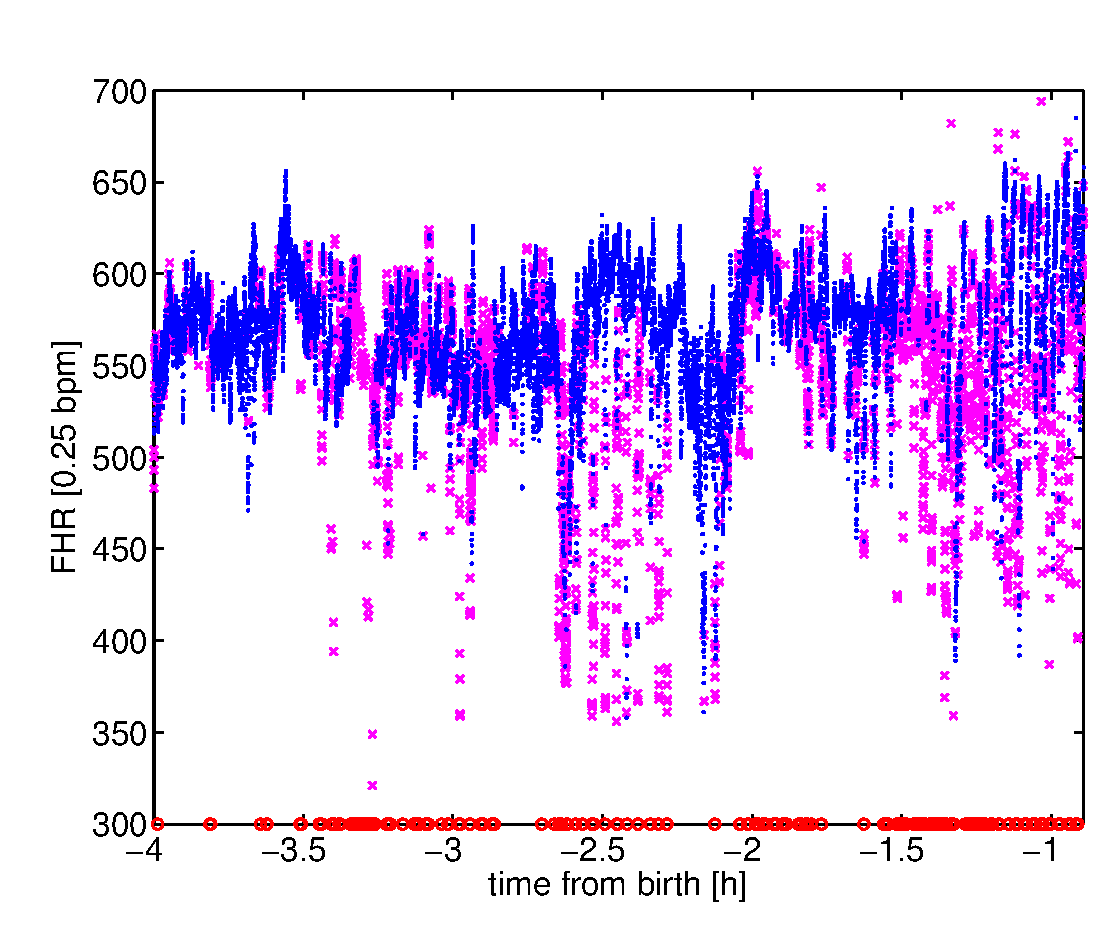
\includegraphics[width=0.9\linewidth]{./figs/caso}}\\%
\subfigure[control]{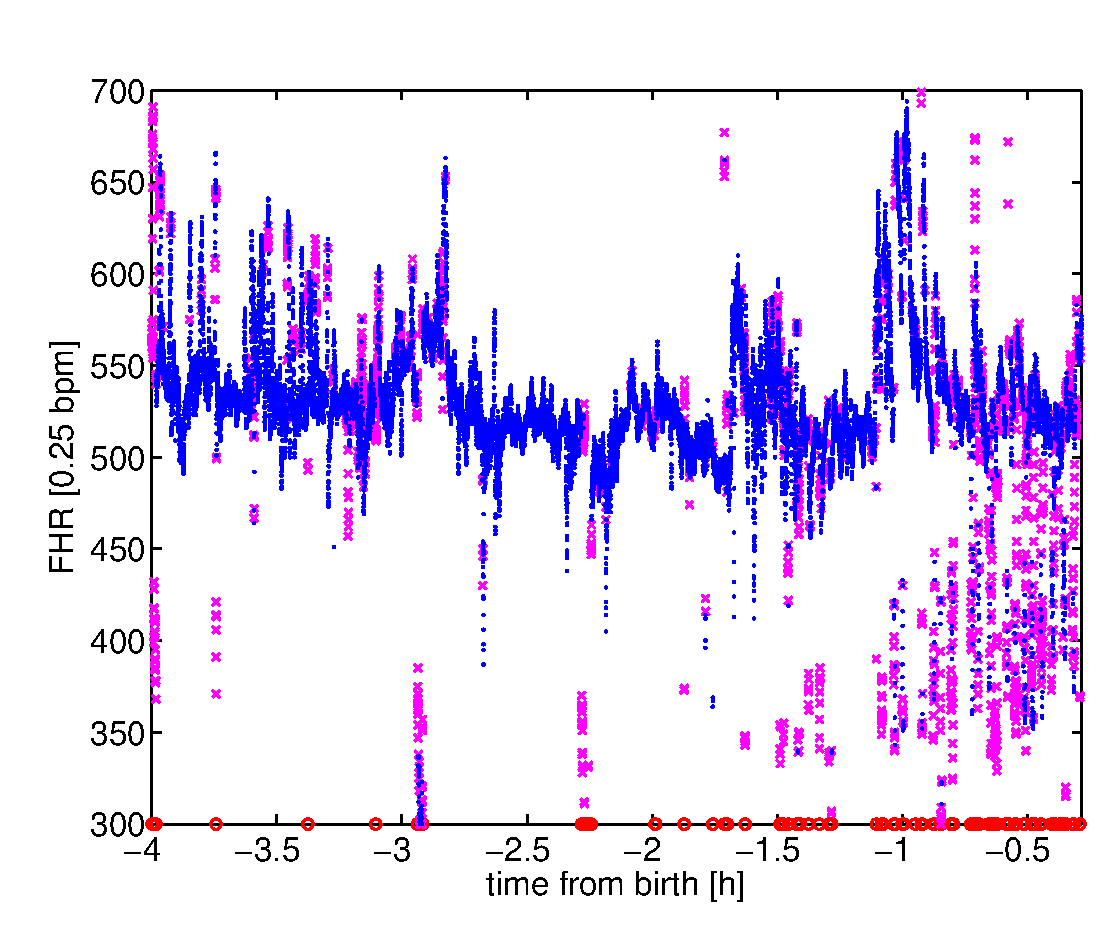
\includegraphics[width=0.9\linewidth]{./figs/control}}
\caption{FHR for (a) a hypoxic and (b) a control patient. Signal qualities are 9.9\% lost, 19.2\% medium and 70.9\% high for (a) ; and 1.8\% lost, 9.8\% medium and 88.3\% high for (b).  Signal qualities  high, medium and lost  are respectively represented by the markers: ``\textcolor{blue}{$\cdot$}'', ``\textcolor{magenta}{x}'' and ``\textcolor{red}{o}''.}
\label{fig:RAWFHR}
\end{figure}
%##########################################################
% Section data description
%##########################################################



% 
%%%Results%%%%%%%%%%%%%%%%%%%%%%%%%%%%%%%%%%
%##########################################################
\section{Results}
%##########################################################
\label{sec:experiments}

The experimental results are presented by following the next sequence:
\begin{itemize}
\item  We started by evaluating the classification performance in FHR records, wihtout any preprocessing, using only the NCD similarity criterion and a nearest neighbor classifier. This experiment evaluated the performance of NCD and set the baseline accuracy that could be attained. 

\item Next, we considered as features for hypoxia classification the aforementioned time and frequency indices that are commonly used in HRV analysis, aiming to evaluate whether they showed some improvement over NCD raw analysis. 

\item Then, we analyzed the performance obtained by using as features the general purpose statistical moments applied to the raw signals. 

\item We also performed feature selection on each group of variables (time and frequency HRV indices and statistical moments), in order to identify the best features and to see whether feature selection could improve classification performance.

\item The experiments continued by evaluating whether the NCD could empower the HRV parameters and statistical moments by obtaining the similarity of the (possibly different length) sequences that result of their application on sliding windows. 

%\item Finally, as the previous experiment only deals with a statistic at a time, we consider feature selection and two strategies (voting classifiers decisions and adding similarities) to combine several statistical moments with the aim of increasing single moment accuracy and yielding more robust results. 

\end{itemize}

\subsection{Raw data analysis}

In this experiment, we analyzed the FHR raw signals in the four time intervals described before. We analyzed three types of signals: a)  including only high quality signals; b) including also medium quality signals; c)  including also medium quality and lost (represented with zeros) signals.

By using NCD, a dissimilarity matrix was created with all pairwise dissimilarities among signals.  We used the software provided by NCD authors~\cite{complearn} to compute the NCD for the signals with three compressor types (zip, bzip2, and lzma). The accuracy was estimated by using LOO cross-validation with a nearest neighbour classifier. 


Best results are summarized in Table~\ref{tab:ncd:raw}, where we can see that high quality signal and the interval from 4 to 3 hours before delivery are the best for prediction accuracy (0.73). In addition, we see that, for the same time interval, the prediction using all the signal is better than using only high and medium qualities, which shows that taking into account lost signals that may occur when the fetus moves, might increase prediction accuracy. Best prediction accuracy for all the patients (4 to 1 hours to delivery interval) was done again considering only high quality signal, but it did not rise above 0.66.

\begin{table}[t]
% DATA from resultadosPrueba_NCD2
\centering
\caption{NCD and nearest neighbor classifier best results for raw signals. ``Quality'' shows the types of signal included in the analysis (High,Medium,Low). ``Interval'' expresses the signal interval in hours to delivery. ``T/C'' shows the number of conTrols and  Cases, respectively. ``Acc.'', ``Sen.'' and ``Spe.'' stand for accuracy, sensitivity and specificity, respectively; and ``Sym.'' shows the method used to make the dissimilarity matrix symmetric.}
\label{tab:ncd:raw}
\resizebox{\linewidth}{!}{\begin{tabular}{cccccccc}
%\toprule
Quality & T/C & Interval & Acc. & Sen. & Spe. & Compressor & Sym.\\ 
%\midrule
H & 13/13 & 4 $\leftrightarrow$  3 & \textbf{0.73} & 0.69 & 0.77 & zip & min\\
H & 13/14 & 3 $\leftrightarrow$  2 & 0.63 & 0.57 & 0.69 & bzip2  & min\\
H & 15/16 & 2 $\leftrightarrow$  1 & 0.58 & 0.75 &0.40  & lzma  & mean\\
H & 15/17 & 4 $\leftrightarrow$  1 & 0.66 & 0.82 & 0.47 & zip & min\\

HM & 13/13 & 4 $\leftrightarrow$  3 & 0.58 & 0.62 & 0.54 & zip & min\\
HM & 13/14 & 3 $\leftrightarrow$  2 & 0.56 & 0.79 & 0.31 & bzip2 & min \\
HM & 15/16 & 2 $\leftrightarrow$  1 & 0.55 & 1.0 & 0.07 & lzma & mean\\
HM & 15/17  & 4 $\leftrightarrow$  1 & 0.56 & 0.59 & 0.53 & lzma & min\\

HML & 13/13 & 4 $\leftrightarrow$  3 &0.66  & 0.77 &0.54  & zip & min\\
HML & 13/14 & 3 $\leftrightarrow$  2 & 0.56 & 0.14 & 1.0 & lzma & min\\
HML & 15/17 & 2 $\leftrightarrow$  1 & 0.53 & 0.76 & 0.27 & lzma & min\\
HML & 15/17 & 4 $\leftrightarrow$  1 & 0.59 & 0.59 & 0.60 & zip & min\\
%\bottomrule
\end{tabular}}
\end{table}

\subsection{Time and frequency HRV indices}

We obtained a set of relevant time HRV descriptors for the considered time intervals. We used all signal qualities, but in this experiment, interpolation was performed on the beats classified as artifacts, as described in Section~\ref{subsec:feat:extraction}. Then, we standardized (zero-mean, unit-variance) each descriptor and combined all of them in a vector.  We benchmarked the following classifiers:  nearest neighbour (NN), $k$ nearest neighbours ($k$-NN), and SVM with linear (SVC) and radial basis function  (RBF-SVC)  kernels. As these features were not designed as dissimilarities, we tried also the SVM,  both to compare its performance with nearest neighbour based classifiers, and to try to extract the best performance of these indices. Table~\ref{tab:time:freq:5min:moments} shows the results of leave one out cross-validation.  The best performance  (0.74 accuracy) was obtained in the 3 $\leftrightarrow$  2 interval by a SVM classifier.


 We repeated the same experiments with the commonly used frequency HRV indices considered above. Results are shown in Table~\ref{tab:time:freq:5min:moments}.  Again, the best results (0.74 accuracy) were obtained in the  3 $\leftrightarrow$  2 interval by k-NN. The combination of the Time and Frequency indices (table not shown) gave a maximum accuracy of 0.70 in the 3 $\leftrightarrow$  2 interval with all classifiers but 1-NN. The best results obtained by these methods provided almost no gain over raw analysis.


\subsection{Statistical Moments}

% + momentos simples.
% prueba_momentos2 y resultado_prueba_momentos2

In order to compute the moments on the records including high and medium signal qualities, we firstly scaled the FHR signal dividing it by the maximum value of each moment for all patients. Then, we calculated raw and central moments of orders $n=\{1,2,\ldots,10\}$ for each patient. Finally, the moments were applied the transformation $x \rightarrow \sqrt[k]{x}$, where $k$ is the order of the moment, and standardized (zero-mean and unit-variance). The results of classifying the records with these moments are also shown in Table~\ref{tab:time:freq:5min:moments}, where a $0.69$ accuracy was obtained in the 4 to 3 hours and in the 4 to 1 hours before delivery intervals. Again, no real gain was obtained by these set of features over the raw analysis.



\begin{table}[t]
%DATA from: prueba_TimeDomain
% DATA from prueba_FreqDomain
% DATA from resultado_prueba_momentos2
\caption{HRV time and frequency indices and statistical moments accuracy for the considered time intervals. SVC and RBF-SVC stand for linear and radial basis kernel Support Vector Classifier, respectively.}
\label{tab:time:freq:5min:moments}
\centering
\begin{tabular}{cccccc}
%\toprule
 Interval          & Features    & 1-NN & $k$-NN & SVC           & RBF-SVC       \\ 
%\midrule
 4 $\leftrightarrow$  3 &Time &0.69 & 0.69   & 0.35          & 0.5           \\ 
 3 $\leftrightarrow$  2 & &0.70 & 0.67   & \textbf{0.74} & \textbf{0.74} \\ 
 2 $\leftrightarrow$  1 & &0.59 & 0.5    & 0.47          & 0.47        \\ 
 4 $\leftrightarrow$  1 & &0.47 & 0.5    & 0.5           & 0.37        \\ 
%\midrule
 4 $\leftrightarrow$  3 &Frequency &0.54 & 0.65          & 0.62 & 0.46    \\
 3 $\leftrightarrow$  2 & &0.56 & \textbf{0.74} & 0.67 & 0.70    \\
 2 $\leftrightarrow$  1 & &0.58 & 0.58          & 0.42 & 0.23    \\
 4 $\leftrightarrow$  1 & &0.5  & 0.5           & 0.53 & 0.44    \\
%\midrule
 4 $\leftrightarrow$3 &Moments &\textbf{0.69}   &   0.62   &   0.46   &   0.58    \\
 3 $\leftrightarrow$2 & &0.22   &   0.63   &   0.59   &   0.52    \\
 2 $\leftrightarrow$1 & &0.23   &  0.065   &   0.48   &   0.29    \\
 4 $\leftrightarrow$1 & & 0.5   &   0.44   &   \textbf{0.69}   &   0.59   \\
%\bottomrule
\end{tabular}
\end{table}




% \subsection{Feature Selection} %% Sin tablas
% Sometimes the learning task can be simplified and even improved by selecting variables. In this section we applied forward selection (FS) to  HRV (time and frequency) indices and to statistical moments. 
% The results of applying  FS to the time HRV indices (table not shown) were in general not better than the obtained without feature selection, maximum overall accuracy decreased to 0.72, which was found in the interval 2 to 1 hours to delivery, where, however, it improved the previous result that was 0.59. FS algorithm consistently selected $stdFHR$  as the unique feature for classification for this case.
% The results (table not shown) for  FS on the frequency HRV indices were slightly better than without feature selection. Best result (0.75 accuracy) was attained on the  4 to 1 hours to delivery interval.  FS algorithm consistently selected $P_{LF}/(P_{MF}+P_{HF})$  as the unique feature for classification for this case. 

% FS on the statistical moments improved the maximum accuracy obtained in Table~\ref{tab:time:freq:5min:moments} with a moderate increase from (0.69 to 0.73). 
% Most selected features for the interval 4 to 3 hours to delivery, where highest accuracy is attained (0.73), were $\mu_4, \mu_8$ and $\mu_9$. 


\subsection{Feature Selection}

Sometimes, the learning task can be simplified and even improved by selecting variables. In this section, we applied forward selection (FS) to  HRV (time and frequency) indices and to statistical moments.   The results of applying  FS to the time HRV indices, shown in Table~\ref{tab:time:freq:5min:moments:featsel}, were in general not better than the obtained without feature selection, as maximum overall accuracy decreased to 0.72, which was found in the interval 2 to 1 hours to delivery, where, however, it improved the previous (0.59) result. FS algorithm consistently selected $stdFHR$  as the unique feature for classification for this case.

The results for FS on the frequency HRV indices, shown in Table~\ref{tab:time:freq:5min:moments:featsel}, were slightly better than without feature selection. FS slightly improved the result in all time intervals. The best result (0.75 accuracy) was attained on the  4 to 1 hours to delivery interval. FS algorithm consistently selected $P_{LF}/(P_{MF}+P_{HF})$  as the single classification feature for this case. 

The results of FS on the statistical moments improved the maximum accuracy obtained in Table~\ref{tab:time:freq:5min:moments} with a moderate increase  (from 0.69 to 0.73). Most selected features for the interval 4 to 3 hours to delivery, where the highest accuracy was attained (0.73), were $\mu_4, \mu_8$, and $\mu_9$. 

\begin{table}[t]
%DATA from: prueba_TimeDomain_featsel
%DATA from: prueba_FreqDomain_featsel
% prueba_momentos_featsel4
% resultado_prueba_momentos_featsel4
\caption{Forward selection accuracy in HRV time and frequency indices and statistical moments for the considered time intervals.}
\label{tab:time:freq:5min:moments:featsel}
\centering
\begin{tabular}{cccccc}
%\toprule
 Interval             &Features  & 1-NN & $k$-NN & SVC           & RBF-SVC       \\ 
%\midrule
 4 $\leftrightarrow$  3 & Time& 0.54  &   0.54  &   0.27   &  0.35 \\
 3 $\leftrightarrow$  2 & & 0.48  &   0.67  &   0.63   &  0.59 \\
 2 $\leftrightarrow$  1 & & \textbf{0.72}  &   0.72  &   0.44   &  0.69 \\
 4 $\leftrightarrow$  1 & & 0.34  &   0.34  &   0.56   &  0.38 \\
%\midrule
 4 $\leftrightarrow$  3 &Frequency &  0.62  &   0.62  &   0.077  &   0.65 \\
 3 $\leftrightarrow$  2 & &  0.52  &   0.59  &   0.74   &   0.67 \\
 2 $\leftrightarrow$  1 & &  0.65  &   0.48  &   0.19   &   0.55 \\
 4 $\leftrightarrow$  1 & &  \textbf{0.75}  &   0.75  &   0.34   &   0.41 \\
5
%\midrule
 4 $\leftrightarrow$  3 & Moments&\textbf{0.73}  &    \textbf{0.73}   &   0.19   &   0.69    \\
 3 $\leftrightarrow$  2 & &0.26  &     0.3   &   0.41   &    0.3    \\
 2 $\leftrightarrow$  1 & &0.42  &    0.39   &   0.42   &   0.42    \\
 4 $\leftrightarrow$  1 & &0.41  &    0.34   &   0.44   &   0.41    \\
%\bottomrule
\end{tabular}
\end{table}
  




\subsection{Time and Frequency Indices in Sliding Windows}

A HRV parameter or a statistical moment provides us with a single value for a signal. If we divide the signal in equal sized windows we got more values, but when comparing  these values with the ones from another patient, both signals should have same length, which will not happen in practice. On the other hand, it is easy to obtain a similarity on signals or sequences of different lengths by using NCD. Therefore, the use of NCD allows us to compare signals from two patients by using the fine grained description provided by the time evolution of a given statistic obtained in a sliding window.
Note that this approach  also evaluates whether  a sequence obtained by sequentially calculating a statistic in a sliding window could have information that can be better exploited by the compressor than the raw signal, which would be(not possible in theory if the  perfect Kolmogorov Complexity could be calculated, but it would be possible in practice as compressors are not perfect.
Therefore, we considered  the calculation of new signals from obtaining these statistics in each time interval of FHR analysis, and we evaluated the performance of obtaining the similarities of these signals for all patients with NCD and by classifying the result with a nearest-neighbour classifier. 


For each time interval, we used the NCD to analyze the time and frequency indices in 5-minute sliding windows, where a window is only considered if its data had not too many artifacts (see Section~\ref{subsec:feat:extraction}). For each parameter, a sequence was constructed for each patient by  concatenating the parameter value for each sliding window of the FHR signal. An NCD matrix for each parameter was later constructed by obtaining the similarities among all pairs of patient sequences, and  the accuracy of a nearest neighbour classifier was estimated by leave-one-out cross-validation.

Table~\ref{tab:ncd:time:freq:moments:5min} shows the best individual accuracies of the HRV time indices in each analysis interval. The best result (0.70 accuracy, 0.86 sensitivity and 0.54 specificity) was again in the  3 $\leftrightarrow$  2 interval by using the LTI index. We combined the 4 time indices by voting, and the best result gave  an accuracy of 0.66 with sensitivity of 0.76 and specificity of 0.53 in the 4 $\leftrightarrow$  1 interval, which was better that the result provided by adding the dissimilarity matrices.


Table~\ref{tab:ncd:time:freq:moments:5min} also shows the best individual accuracies of the HRV frequency indices. The best result (0.77 accuracy, 0.77 specificity and 0.77 specificity) was in the  4 $\leftrightarrow$  3 interval by using $P_{LF} / (P_{MF}+P_{HF})$. Different indices seemed to be the most informative in each interval. We combined the 6 frequency indices by adding the dissimilarity matrices, and the best result gave an accuracy of 0.69 with sensitivity of 0.53  and specificity of 0.85 in the 4 $\leftrightarrow$  3 interval.

\begin{table}[t]
% DATA from prueba_momentos_5min.mat
\caption{NCD and nearest neighbour classifier best results for HRV time and frequency indices and statistical moments in 5-minute sliding-windows signals.}
\label{tab:ncd:time:freq:moments:5min}
\centering
\begin{tabular}{cccccccc}
%\toprule
 Interval    &Features   & Acc.     & Sen. & Spe. & Feature  & Comp. & Sym. \\ 
%\midrule
 4 $\leftrightarrow$  3 & Time & 0.62 &0.69 & 0.54 &  $sdFHR$ & bzip2 & min\\
 3 $\leftrightarrow$  2 & &\textbf{0.70} &0.86 & 0.54 &  LTI & lzma & min\\
 2 $\leftrightarrow$  1 & & 0.66 &0.65 & 0.67 & \mfhr & bzip2 & min\\
 4 $\leftrightarrow$  1 & & 0.69 & 0.76 & 0.6 & \mfhr & bzip2 & min\\
%\midrule
 4 $\leftrightarrow$  3 & Frequency& \textbf{0.77} & 0.77 & 0.77 & $\frac{P_{LF}}{P_{MF}+P_{HF}}$ & bzip2 & min\\
 3 $\leftrightarrow$  2 & & 0.59 & 0.64 & 0.54 & $P_{VLF}$ & bzip2 & min\\
 2 $\leftrightarrow$  1 & & 0.69 & 0.65 & 0.73 & $P_{HF}$ &  bzip2 & min\\
 4 $\leftrightarrow$  1 & & 0.69 & 0.88 & 0.47 &$P_{LF}$ & lzma & mean\\  
%\midrule
%acc3
 4 $\leftrightarrow$  3 & Moments& \textbf{0.88} & 0.92 & 0.85 & $\mu_3$ & lzma       & min    \\
%acc2
 3 $\leftrightarrow$  2 & & 0.70          & 0.64 & 0.77 & $\mu_2$ & bzip2      & min    \\ % tambien (\mu_2,bzip2, mean) y (M_8, zip, mean)
% acc1
 2 $\leftrightarrow$  1 & & 0.77          & 0.81 & 0.73 & $M_4$  & zip        & mean    \\ % tambien (\mu_9,lzma,min)
%acc4
 4 $\leftrightarrow$  1 & & 0.81          & 0.82 & 0.80 & $M_4$  & lzma       & mean    \\ 
%\bottomrule
\end{tabular}
\end{table}


\subsection{Moments in Sliding Windows}

In this experiment, we used high and medium signal qualities and 5 minutes sliding windows. For each window, we computed raw and central moments of orders $n \in \{1,2,\ldots,10\}$. Then, for each moment of order $n$, the results of all windows were concatenated to obtain the new signal $\bs_{i,n}$ that provided a description of the patient $i$. Later, this signal was transformed as $\bar{\bs}_{i,n}=\sqrt[n]{\bs_{i,n}}/A_n$ where  $A_n$ is the maximum value of the signals $\{\bar{\bs}_{i,n}\}_{i=1}^{N_T}$. Then, the NCD pairwise distances were obtained for pairs $(\bar{\bs}_{i,n}, \bar{\bs}_{j,n})$ and accuracies were estimated using leave-one-out cross-validation with a nearest neighbour classifier.

The results are summarized in Table~\ref{tab:ncd:time:freq:moments:5min}. The best predictive interval was the 4 to 3 hours to delivery. The best accuracy for individual moments gave an accuracy of 0.88  (23 out of 26), a sensitivity of 0.92 (12 out of 13) and a specificity of 0.85 (11 out of 13). In addition, we noted the good performance of the 4 to 1 hours to delivery interval, which  can be applied to any record of our database, 0.81 accuracy (26 out of 32), 0.82 sensitivity (14 out of 17) and 0.80 specificity (12 out of 15).




%\subsection{Voting moments in sliding windows}
%One possibility to increase accuracy is to combine the decisions of independent experts. An expert, in this case, is a classifier that uses the NCD similarities calculated from one statistical moment. Table~\ref{tab:ncd:time:freq:moments:5min} shows the best moments for each time interval. We combined decisions from the intervals 4 to 3 hours,  3 to 2 and 2 to 1 hours to delivery for the records that have signal in the three interval (25 in our case). 
% Feature selection with the methods presented above was applied to the training data inside each LOO cross-validation step to select the decisions (moments) to be combined. 
%The results for these methods with a nearest neighbor classifier are summarized in Table~\ref{tab:fs:momentos:comp:voting:adding}. We note that there were 120 variables (20 moments, 3 compressors, and 2 ways of considering the dissimilarity matrix) for the one-hour intervals (360 for the three hours interval) and 25 instances to classify, which made the feature selection problem hard and  prone to overfitting. The maximum number variables to be searched by forward selection was limited to five, in order to limit the overfitting effect.
%Best result, 0.73 accuracy,  was provided  by the 4 to 3 hours to delivery interval. This result did not reach the accuracies presented above, and the feature selection methods were not able to find the best variables (maximum accuracy could reach 0.96 picking variables by hand). The more selected moments in each loop step are detailed  in decreasing order of appearance as follows: $\mu_3$, $M_1$, $M_{10}$, $M_9$, $\mu_4$, $\mu_6$ (variables only selected once are omitted). To compute the nearest neighbor, the \emph{min} matrix type was selected in the majority of cases. The type or compressor more selected was lzma, then bzip2, and finally zip.


%\subsection{Combining moment dissimilarity matrices}

%Voting can be understood as a simple combination of hard decisions, because we ignore how \emph{sure} the classifier is about its vote. Another possibility is to combine soft decisions, which in our case is equivalent to the addition of the dissimilarity matrices previous to   the nearest neighbor classification (the moment matrices to be added are determined by feature selection). By using soft decisions, a case that is going to be wrongly classified by one variable could be corrected by another variable that has a greater confidence about this case. It may also happen the converse, a confident but wrong opinion can hinder a good classification. To compare both methods, we present the results for the addition of dissimilarity matrices in Table~\ref{tab:fs:momentos:comp:voting:adding}. Best results (0.88 accuracy, 0.85 sensitivity, 0.92 specificity)  were given for the FS feature selection method, in the 4 to 1 hours to delivery interval. Most selected variables were in this case: $\mu_3$, $M_1$ ,$M_{10}$ and $M_9$ (variables only selected once are omitted). All variables were selected from the min type of matrix. The type or compressor more selected was bzip2, then lzma, and finally zip.



%\begin{table}[t]
%  \caption{LOO cross-validation accuracy given by nearest neighbor classifier and two feature selection procedures for moment signals in 5 minutes sliding windows combining variables by voting classifier decisions or adding dissimilarity matrices.}
%  \label{tab:fs:momentos:comp:voting:adding}
%  \centering
%  \begin{tabular}{ccccc}
%\toprule
%                        & \multicolumn{2}{c}{Voting} & %\multicolumn{2}{c}{Adding}                                        \\
% \cmidrule(r){2-3}   \cmidrule(r){4-5}
%                                               & ATS   & FSCV2          & ATS   %& FSCV2 \\
%\midrule
% 4 $\leftrightarrow$  3                        & 0.58  & \textbf{0.73}  & 0.81  %& 0.58  \\
% 3 $\leftrightarrow$  2                        & 0.41  & 0.41           & 0.37  %& 0.63  \\
% 2 $\leftrightarrow$  1                        & 0.61  & 0.71           & 0.48  %& 0.55  \\
% 4 $\leftrightarrow$  1                        & 0.52  & 0.68           & 0.76  %& \textbf{0.88}  \\
%\bottomrule
%  \end{tabular}
%\end{table}





\section{Discussion and Conclusions}
\label{sec:discussion}

\myblue{Several indices have been proposed to analyze FHR. The most common indices are based on time domain and frequency domain methods~\cite{Signorini:2003ee,vanLaar:2009dj}. Time domain methods aim to assess the long and short term variability of the FHR, whereas frequency domain methods aim to characterize the oscillatory contributions on the FHR. In many cases these indices are reduced to a single number obtained in the entire time series or to a collection of numbers obtained in 5-minute windows slides, which are again reduced to a few numbers like mean or standard deviation. }

We have proposed NCD as a similarity measure for FHR registers because it is able to exploit both linear and non-linear relations among records. We tried it with raw FHR records, time and frequency indices and moments signals extracted from sliding windows. We obtained better performance from the moments than from the raw records, which shows that the compressor is not able to extract all the relations in the data and preprocessing might help. Then, we have shown how to combine several moments (or other type of variable) by using a simple voting scheme and by summing the dissimilarity matrices, which provide overall better results in our case.

Main strengths of using NCD for comparing FHR registers or signals of  any statistic applied to signal windows are simplicity and generality. Other commonly used information-theoretical measures, like Approximate entropy~\cite{Pincus1991} or Sample entropy~\cite{Richman2000}, need to tune the embedding dimension and specially the tolerance, which is a continuous parameter; but there is no parameter to tune for our approach. Indeed, despite we have tried three compressors and two simple approaches to get a symmetric matrix  the proposed methodology can be straightforwardly used with a lzma compressor and the min approach to get symmetric NCD matrices.  In addition, there is no problem with the common signal losses, which is a problem to apply frequency-related methods as they need signal interpolation, which is not always possible. The similarity can always be computed independently of how the signal losses are addressed. 

\myblue{{\it Visual interpretation} values  basal FHR, its accelerations and decelerations in relation to uterine contractions, and beat-to-beat FHR variability~\cite{Ayres-de-Campos2010a,RajendraAcharya2006}.
The following signal types are considered clearly pathological (suspicious of hypoxia): late decelerations, whose nadir has a delay of at least 30 seconds with respect to the acme of contractions; maintained bradycardia;  low variability (less than 5 beats); and a ``sine''-rhythm, named after its wave-like appearance, which is characterized by a long-term variability but almost no variability in the short-term.}

\myblue{First, late decelerations are produced in the following manner. During uterine contraction, when the myometrium pressure exceeds the blood pressure of the intervillous space of the placenta, maternal circulation is interrupted and therefore ceases to carry oxygen to the fetal territory. In a well oxygenated fetus, this is not a problem since the fetus does not consume all the tissue-oxygen before the end of the contraction. In a fetus with poor oxygenation, on the other hand, the oxygen reserves are exhausted before the end of contraction and, particularly in the more sensitive heart cells (which act as a pacemaker), action-potential production mechanisms are delayed, which causes bradycardia.}

\myblue{And second, the decrease in variability is more difficult to explain. On the one hand,  the regulation of FHR, usually controlled by the vagus nerve, is stopped by cardiac and nervous system hypoxia. On the other hand,  it seems that there are less functionally active cells in the pacemaker as the hypoxia progresses. The regulatory system loses ``degrees of freedom'', which therefore becomes increasingly uniform and deterministic~\cite{Goldberger1987}.
}

\myblue{FHR signal can be measured in two ways, namely, external, by using a ultrasonic sensor that observes the Doppler effect; and internal, in which fetal electrocardiogram (ECG) is measured with an electrode in the fetus scalp. Uterine activity can also be measured in two ways: by  using a non-invasive pressure transducer in the mother's abdomen, or with an invasive intrauterine catheter pressure sensor}.

\myblue{Automatic analysis of CTG has also been proposed. In \cite{AMERWAHLIN2001}, automatic ST analysis (the ST segment connects the QRS complex and the T wave) combined with CTG was shown to increase the ability of obstetricians to identify hypoxia and to improve the perinatal outcome. In \cite{Ayres-de-Campos2010},  a clinical trial was proposed to assess whether computer analysis and alerts improves visual CTG monitoring. A system-identification approach was proposed \cite{Warrick2010} to model FHR and uterine activity as an input-output system,  reporting around 50\% sensitivity with 7.5\% of false positives at 1h and 40 minutes before delivery.  Time-frequency analysis and features from time-frequency space decomposition were sucessfully used in an animal study yielding  93\% sensitivity  and 98\% specificity\cite{Dong2014}.
Other non-invasive approaches have been proposed to complement CTG, such as Doppler velocimetry and pulse oximetry~\cite{Yang1998,Siristatidis2004,Mori2014}, or  near-infrared spectroscopy to measure cerebral metabolic rate of oxygen~\cite{Tichauer2009}. The performance of automatic approaches currently applied to hypoxia detection has still room for improvement both in accuracy (sensitivity and specificity) and in the time before birth where hypoxia is detected.}

\myblue{NCD technique was successfully used for clustering the fetuses of a multicentric study with the aim of identifying the abnormal ones~\cite{CostaSantos2006}. }

It is remarkable that, using sliding windows and NCD, both frequency indices and moments obtain the best accuracies in the  4 $\leftrightarrow$  3 hours interval whereas time indices obtain the best results in the  3 $\leftrightarrow$  2 hours interval. Our comparisons show that the commonly used Time and Frequency indices can be complemented by the moments, which are always applicable and do not suffer from signal loses. In addition, fetus movement might provide valuable information as we noted when analyzing raw signals (Table~\ref{tab:ncd:raw}), and when we observed the performance of $P_{LF} / (P_{MF}+P_{HF})$ index, which depends on fetus movement (Table~\ref{tab:ncd:time:freq:moments:5min}). Finally, by adding similarity matrices selected by FS a promising 0.88 accuracy is reached in the 4 $\leftrightarrow$  1 hours interval, which compares entire records and mimics the processing of a fetus during labor.

Practical implementation of this approach as an plugin of the available CTG systems is straightforward. We recommend to perform a careful selection and labeling of FHR records. Then, the number of cases in the knowledge database and processing capabilities must be balanced. For instance, the  analysis of an FHR record every minute against a knowledge database of 1000 patients is easily done in a normal PC using gzip as compressor.

%% JL: Creo que sería muy bueno que Carlos escribiera uno o dos párrafos de discusión y conclusiones.
 
%+ 1 párrafo o dos Discusión Carlos.

%\section{Conclusions}

The decision making during the labor is a difficult task for the gynecologist. It always should be intended to be as less invasive as possible, but, of course, ensuring fetal well-being and acting as soon as possible in case of  suspicion of fetal hypoxia. Our main contribution shows how the NCD analysis of the readily available FHR traces may help the gynecologists to make the correct decisions. We reach 88\% accuracy, which is a remarkable result if we take into account that we are actually identifying stressed fetuses 3 hours before delivery that were not detected by the gynecologist until a later stage.
This general methodology is also applicable to other time series classification problems and it is both simple to understand and simple to apply.

The results obtained in this study indicate that a further study with more patients should be performed to open the application of this type of FHR analysis of the fetus condition to the industry.
\section*{Acknowledgements}
The author \'Oscar Barquero P\'erez has the support of a FPU Grant (AP2009-1726) from the Ministerio de Educaci\'on, Spanish Government. Authors want to thanks professor Antonio Garc\'ia Marques for his suggestions and thoughtful comments on LASSO models.
\bibliography{./bib/neonatos-abrv.bib}
%% 
\begin{correspondence}
O Barquero-P\'erez\\
Department of Signal Theory and Communications\\
University Rey Juan Carlos. B104, Camino del Molino s/n\\
28943 - Fuenlabrada (Madrid), Spain\\
Phone: +34 91 488 84 62\\
oscar.barquero@urjc.es
 \end{correspondence}

\end{document}